% Author: Izaak Neutelings (July, 2017)

\documentclass[border=3pt,tikz]{standalone}
\usepackage{amsmath} % for \dfrac
\usepackage{tikz}
\tikzset{>=latex} % for LaTeX arrow head
\usepackage{pgfplots} % for the axis environment
\usetikzlibrary{calc} % to do arithmetic with coordinates
\usetikzlibrary{angles,quotes} % for pic

% colors
%\definecolor{mylightblue}{RGB}{170,170,230}
\definecolor{mylightgrey}{RGB}{230,230,230}
\definecolor{mygrey}{RGB}{190,190,190}
\definecolor{mydarkgrey}{RGB}{110,110,110}
\definecolor{mygreen}{RGB}{120,220,160}
\definecolor{mydarkgreen}{RGB}{60,120,60}
\definecolor{myverydarkgreen}{RGB}{20,60,20}
\definecolor{mydarkred}{RGB}{140,40,40}
\definecolor{mylightblue}{RGB}{220,228,255}
\definecolor{myblue}{RGB}{183,191,229}
\definecolor{mydarkblue}{RGB}{50,70,190}
\definecolor{mygold}{RGB}{250,200,80}

% mark right angle
\newcommand{\MarkRightAngle}[4][1.5mm]
{\coordinate (tempa) at ($(#3)!#1!(#2)$);
 \coordinate (tempb) at ($(#3)!#1!(#4)$);
 \coordinate (tempc) at ($(tempa)!0.5!(tempb)$);%midpoint
 \draw (tempa) -- ($(#3)!2!(tempc)$) -- (tempb);
}

\begin{document}


% RUTHERFORD SCATTERING
\begin{tikzpicture}[scale=1]
% https://tex.stackexchange.com/questions/45151/format-numbers-as-a-fraction-of-pi-with-tikz-pgfmathprintnumber
  
  % limits & parameters
  \def\xa{-2.4}
  \def\xb{ 4}
  \def\ya{-4}
  \def\yb{ 4}
  \def\tmax{2.1}
  \def\a{1.3}
  \def\b{1}
  \def\c{{sqrt(\a^2+\b^2)}}
  \def\N{50} % number of points
  
  % coordinates
  \coordinate (O)  at (   0,  0 );
  \coordinate (A)  at (  \a,  0 );
  \coordinate (F1) at (  {sqrt(\a^2+\b^2)},   0 );
  \coordinate (F2) at ( -{sqrt(\a^2+\b^2)},   0 );
  \coordinate (P)  at ( -{\a^2/sqrt(\a^2+\b^2)}, -{\a*\b/sqrt(\a^2+\b^2)} );
  \coordinate (P1) at (\xb*\a, \yb*\b);
  \coordinate (P2) at (\xb*\a,-\yb*\b);
  \coordinate (yshift) at (0,0.4);
  
  % axes & asymptotes
  \draw[mygrey] % x axis
    (\xa*\a,0) -- (\xb*\a,0);
  %\draw[mylightgrey] % y axis
  %  (0,\ya*\b) -- (0,\yb*\b);
  \draw[dashed,mydarkgrey]
    (-\xb*\a*0.45, \ya*\b*0.45) -- (\xb*\a, \yb*\b)
    (-\xb*\a*0.45,-\ya*\b*0.45) -- (\xb*\a,-\yb*\b);
    
  % arrows
  \def\vtheta{30}
  \def\vradius{0.8}
  \draw[->,myverydarkgreen,shift=($(P1)-(yshift)$),scale=0.6]
	(0,0) -- (-\a,-\b) node[midway,below right=0pt] {${v}_i$};
  \draw[->,myverydarkgreen,shift=($(P2)+(yshift)$),scale=0.6]
	(-\a,\b) -- (0,0) node[midway,above right=-2pt] {${v}_f$};
  \draw[->,myverydarkgreen]
    (\a+0.35,{\vradius*sin(\vtheta)}) arc (180-\vtheta:180+\vtheta+10:\vradius)
    node[above right=0pt] {$v^*$};
  
  % angles
  \MarkRightAngle{F2}{P}{O}
  \pic [draw,myverydarkgreen,"$\theta$",angle radius=12,angle eccentricity=1.4] {angle = F2--O--P};
  \pic [draw,below,angle radius=16,angle eccentricity=1.4] {angle = P2--O--P1};
  \node[right=1pt,below=-2pt,myverydarkgreen] at ($(O)!0.5!(A)$)  {\small$\phi$};
  %\pic [draw,"$\theta$",angle radius=12,angle eccentricity=1.4] {angle = A--O--P1};
  %\pic [draw,"$\theta$",angle radius=15,angle eccentricity=1.4] {angle = P2--O--A};
  
  % hyperbola
  \draw[color=mylightgrey,line width=0.5,samples=\N,smooth,variable=\t,domain=-\tmax*0.58:\tmax*0.58] % left
    plot({-\a*cosh(\t)},{\b*sinh(\t)});
  \draw[color=mydarkgreen,line width=1,samples=\N,smooth,variable=\t,domain=-\tmax:\tmax] % right
    plot({ \a*cosh(\t)},{\b*sinh(\t)}); % {exp(\y)+exp(-\y)
  
  % nodes
  \draw[myverydarkgreen]
    (F2) -- (P) node[midway,below left=1pt,] {$b$};
  \fill[radius=1.5pt]
  	%(F1) circle node[above] {F}
    (A)  circle node[above left=0pt] {A}
    (O)  circle node[above=2pt] {O};
  \fill[radius=2.5pt,mydarkred]
    (F2) circle node[above=2pt] {N};
  \draw[]
    %(O) -- (F2)
    node[left=1pt,above=0pt] at ($(F2)!0.5!(O)$) {$c$}
    node[below right] at ($(P)!0.5!(O)$)  {$a$};
  
  % alpha particle
  \draw[radius=1pt,mydarkgreen,fill]
    ({ \a*cosh(\tmax*1.02)},{\b*sinh(\tmax*1.02)}) circle node[above right=0pt] {$\alpha$};
  
  
\end{tikzpicture}


% RUTHERFORD SCATTERING - shot at center
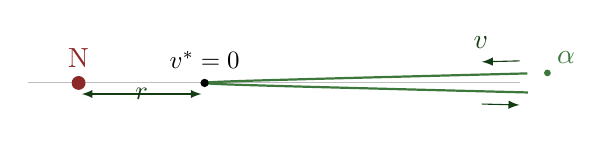
\begin{tikzpicture}[scale=1]
% https://tex.stackexchange.com/questions/45151/format-numbers-as-a-fraction-of-pi-with-tikz-pgfmathprintnumber
  
  % limits & parameters
  \def\xa{-1.8}
  \def\xb{ 6}
  \def\ya{-4}
  \def\yb{ 4}
  \def\a{0.8}
  \def\b{0.02}
  \def\tmax{2.5}
  \def\c{{sqrt(\a^2+\b^2)}}
  \def\N{100} % number of points
  
  % coordinates
  \coordinate (O)  at (   0,  0 );
  \coordinate (A)  at (  \a,  0 );
  \coordinate (F2) at ( -{sqrt(\a^2+\b^2)},   0 );
  \coordinate (P1) at (\xb*\a, \yb*\b);
  \coordinate (P2) at (\xb*\a,-\yb*\b);
  \coordinate (yshift) at (0,0.2);
  
  % axes & asymptotes
  \draw[mygrey] % x
    (\xa*\a,0) -- (\xb*\a,0);
    
  % arrows
  \def\vtheta{30}
  \def\vradius{0.8}
  \draw[->,myverydarkgreen,shift=($(P1)+(yshift)$),scale=0.6]
	(0,0) -- (-\a,-\b) node[midway,above left=1pt] {$v$};
  \draw[->,myverydarkgreen,shift=($(P2)-(yshift)$),scale=0.6]
	(-\a,\b) -- (0,0); node[midway,below right=0pt] {}; %${v}_f$
  
  % hyperbola
  \draw[color=mydarkgreen,line width=0.8,samples=\N,variable=\t,domain=-\tmax:\tmax]
    plot({ \a*cosh(\t)},{\b*sinh(\t)});
  
  % nodes
  \fill[radius=1.5pt]
    (A)  circle node[above=2pt,scale=0.9] {$v^*=0$};
  \fill[radius=2.5pt,mydarkred]
    (F2) circle node[above=2pt] {N};
  \draw[<->,myverydarkgreen,transform canvas={yshift=-4pt,scale=0.95}]
  	(F2) -- (A)
    node[midway] {$r$}
    node[]      at ($(0,-\b*30)$) {};
  
  % alpha particle
  \draw[radius=1pt,mydarkgreen,fill]
    ({ \a*cosh(\tmax*1.02)},{\b*sinh(\tmax*1.02)}) circle node[above right=0pt] {$\alpha$};
  
  
\end{tikzpicture}


% RUTHERFORD SCATTERING - observation
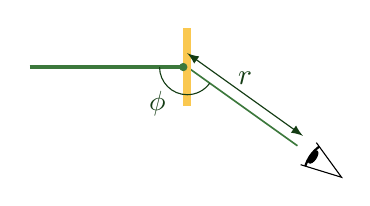
\begin{tikzpicture}[scale=1]
  
  % limits & parameters
  \def\xa{-2.0}
  \def\xb{ 1.4}
  \def\ya{-1}
  \def\yb{ 1}
  \def\h{0.50} % rectangle height
  \def\w{0.05} % rectangle width
  
  % coordinates
  \coordinate (B)  at (\xa,  0 );
  \coordinate (O)  at (  0,  0 );
  \coordinate (M)  at (\xb,-\yb);
  \coordinate (P)  at (\xb*1.142  ,-\yb*1.142);
  \coordinate (E0) at (\xb*1.4    ,-\yb*1.4  );
  \coordinate (E1) at (\xb*1.1-0.1,-\yb*1.1-0.1*\xb/\yb);
  \coordinate (E2) at (\xb*1.1+0.1,-\yb*1.1+0.1*\xb/\yb);
  
  % beams
  \draw[mydarkgreen,line width=1.5]
    (B) -- (O);
  \draw[mydarkgreen,line width=0.6]
    (O) -- (M);
  \fill[mygold] (-\w,-\h) rectangle (\w,\h);
  \fill[radius=1.5pt,mydarkgreen]
    (-\w,0) circle node {};
  
  % angles & distance
  \draw[<->,myverydarkgreen,transform canvas={yshift=5pt,scale=1.05}]
  	(O) -- (M) node[midway,above] {$r$};
  \pic [draw,myverydarkgreen,left=2pt,"$\phi$",angle radius=10,angle eccentricity=1.4] {angle = B--O--M};

  % eye
  \draw[] (E1) -- (E0) -- (E2);
  \pic [draw,thick,angle radius=13.7,angle eccentricity=1.4] {angle = E2--E0--E1};
  \draw[rotate=-34,fill] (P) ellipse (0.04 and 0.09);

\end{tikzpicture}


% RUTHERFORD SCATTERING - hyperbola triangle
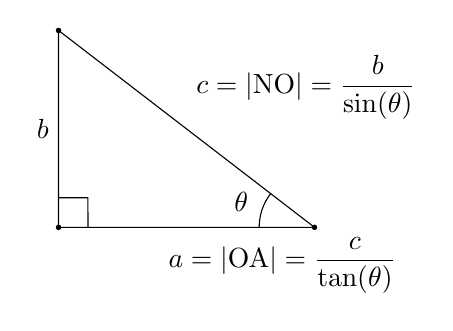
\begin{tikzpicture}[scale=2.5]
% https://tex.stackexchange.com/questions/45151/format-numbers-as-a-fraction-of-pi-with-tikz-pgfmathprintnumber
  
  % limits
  \def\a{1.3}
  \def\b{1}
  
  % coordinates
  \coordinate (O)  at (   0,  0 );
  \coordinate (A)  at ( -\a,  0 );
  \coordinate (B)  at ( -\a, \b );
  
  \fill[radius=0.4pt]
    (A) circle node {}
    (O) circle node {}
    (B) circle;
  
  % lines
  \draw[]
    (O) -- (A) node[midway,left=10pt,below right] {$a = |\text{OA}|=\dfrac{c}{\tan(\theta)}$}
        -- (B) node[midway,left]  {$b$}
        -- (O) node[midway,above right=0pt] {$c=|\text{NO}|=\dfrac{b}{\sin(\theta)}$};

  % angles
  \MarkRightAngle{B}{A}{O}
  \pic [draw,"$\theta$",angle radius=20,angle eccentricity=1.4] {angle = B--O--A};    
  
\end{tikzpicture}


% RUTHERFORD SCATTERING - hyperbolic orbits with different impact parameters
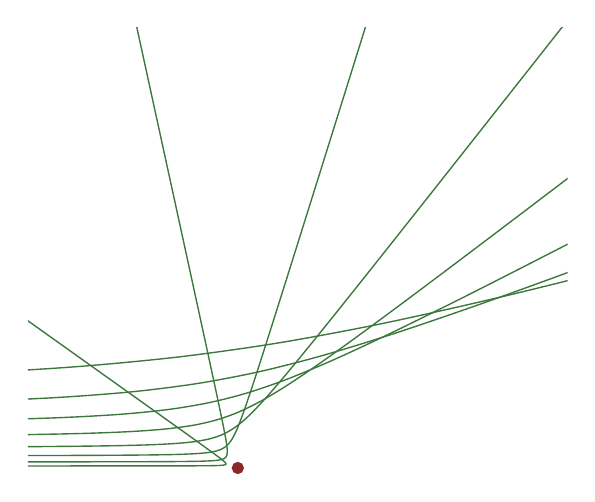
\begin{tikzpicture}[scale=1]
% https://tex.stackexchange.com/questions/45151/format-numbers-as-a-fraction-of-pi-with-tikz-pgfmathprintnumber
  
  % limits & parameters
  \def\xa{-35}
  \def\xb{ 55}
  \def\ya{ -1}
  \def\yb{ 55}
  \def\tmax{5}
  \def\N{30} % number of points
  
  \begin{axis}[ xmin=\xa,xmax=\xb,
                ymin=\ya,ymax=\yb,
                hide x axis, hide y axis,
              ]
    \def\a{1}
    \foreach \u in {1,3,6,10,15,21,28,38}{
      \def\b{\u*0.25}
      \def\c{sqrt(\a^2+\b^2)}
      \addplot[color=mydarkgreen,line width=0.5,samples=\N,smooth,variable=\t,domain=-\tmax:\tmax]
         ({   \a/\c*(-\a*cosh(\t)-\c) + \b/\c*\b*sinh(\t)  },
          {  -\b/\c*(-\a*cosh(\t)-\c) + \a/\c*\b*sinh(\t)  });
    }
    
    \addplot[mydarkred,mark=*,mark size=2pt,mark options=solid] coordinates {(0,0)};
    
  \end{axis}
  
\end{tikzpicture}


% RUTHERFORD SCATTERING - single vs. compound scattering
% http://www.ffn.ub.es/luisnavarro/nuevo_maletin/Rutherford%20(1911),%20Structure%20atom%20.pdf
% https://tex.stackexchange.com/questions/45151/format-numbers-as-a-fraction-of-pi-with-tikz-pgfmathprintnumber
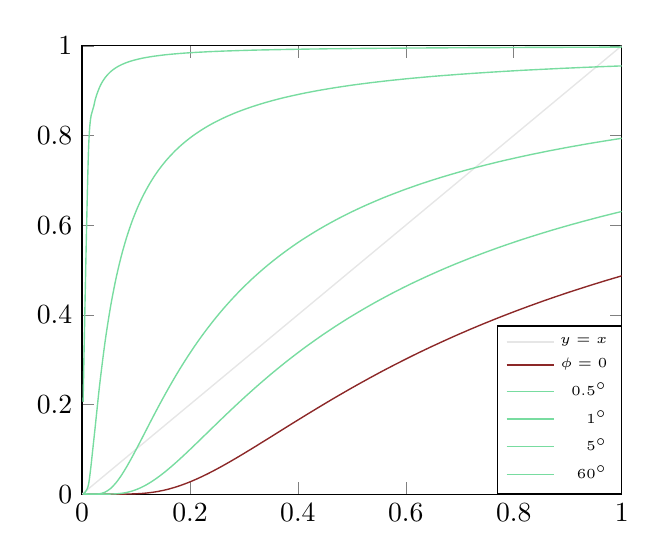
\begin{tikzpicture}[scale=1]
  
  % limits & parameters
  \def\xa{ 0.0}
  \def\xb{ 1.0}
  \def\ya{ 0.0}
  \def\yb{ 1.0}
  \def\A{  1.0}
  \def\B{  1.0}
  \def\N{100} % number of points
  
  \begin{axis}[ xmin=\xa,xmax=\xb,
                ymin=\ya,ymax=\yb,
                legend cell align=right,
                legend style={
                  at={(1.0,0.0)},
                  anchor=south east,
                  font=\fontsize{5}{6}\selectfont}
              ]
    \addplot[color=mylightgrey,line width=0.5,samples=2,variable=\x,domain=0:1]
      (\x,\x);
    \addlegendentryexpanded{$y=x$}
    
    \addplot[color=mydarkred,line width=0.5,samples=\N,variable=\px,domain=0:1]
      ({ \px },{ \A*exp(-0.72/(\B*\px)) });
    \addlegendentryexpanded{$\phi=0$}
    
    \foreach \angle in {0.5,1,5,60}{
      \def\myphi{pi*\angle/180}
      \addplot[color=mygreen,line width=0.5,samples=\N,smooth,variable=\px,domain=0.002:1]
        ({ \px },{ \A*exp(-0.181*\myphi^2*cot(\myphi/2 r)^2/(\B*\px)) }); %*cot(\phi/2)^2
      \addlegendentryexpanded{\angle$^\circ$}
      %\addplot[color=mygreen,line width=0.5,samples=\N,smooth,variable=\px,domain=0:1,forget plot]
      %  ({ \px },{ exp(-0.181*\myphi^2*cot(\myphi/2 r)^2/\px) }); %*cot(\phi/2)^2
    }
    
  \end{axis}
  
\end{tikzpicture}


\end{document}
